%
%  infochimps.tex
%
%  Created by Drew Conway on 2010-12-07
% 
%
\documentclass[xcolor=dvipsnames, 9pt]{beamer}

\newenvironment{code}{\begin{semiverbatim} \begin{footnotesize}}
{\end{footnotesize}\end{semiverbatim}}

\usepackage{graphicx}
\usepackage{amssymb}
\usepackage{amsfonts}
\usepackage{amsmath}
\usepackage{hyperref}
\usepackage{natbib}
\usepackage{color}
\usepackage{pdfsync}
\usepackage{chancery}
\usepackage{movie15}
\usepackage{pgfpages}
\usepackage{fancyvrb}
\usepackage{colortbl}
\usepackage{listings}

% \definecolor{white}{rgb}{255,255,255}
% \definecolor{darkred}{rgb}{0.5,0,0}
% \definecolor{darkgreen}{rgb}{0,0.5,0}
% \definecolor{lightblue}{rgb}{0,0,0.7}

% \hypersetup{colorlinks,
%   linkcolor=white,
%   filecolor=darkred,
%   urlcolor=lightblue,
%   citecolor=darkblue}

\usepackage{beamerthemesplit}
\usetheme{Warsaw}
\usecolortheme[named=Tan]{structure} 
\setbeamertemplate{navigation symbols}{}
\setbeamertemplate{itemize items}[triangle]
\setbeamertemplate{enumerate items}[default]
%\setbeameroption{show notes on second screen}
%\logo{\includegraphics[width = 2cm]{nyulogo.png}}

\newcommand{\R}{\mathbb{R}}
\renewcommand{\d}{\mathsf{d}}
\newcommand{\dd}{\partial}
\newcommand{\E}{\mathsf{E}}
\newcommand{\bb}{\mathbf}

\title{How To Be a Real Data Monkey\\Hacking the Infochimps API with R}
\author{Drew Conway}
\date{December 16, 2010}

\begin{document} 

\begin{frame}[plain]
  \titlepage  
\end{frame}

\begin{frame}
	\frametitle{Introduction}
	\begin{columns}
        \column{.5\textwidth}
            What is infochimps?
            \begin{itemize}
                \item Data clearinghouse
                \item API
            \end{itemize}
            The \texttt{infochimps} R package
            \begin{itemize}
                \item Basic usage framework
                \item Looking at the guts
            \end{itemize}
            Examples
            \begin{itemize}
                \item Geo-location of blog hits
                \item Programming language mentions on Twitter
            \end{itemize}
        \column{.5\textwidth}
            
\includegraphics[width=5.5cm]{images/monkeys.jpg}
	\end{columns}
\end{frame}

\section{Introduction to Infochimps} % (fold)
\label{sec:introduction_to_infochimps}

\begin{frame}[fragile]
    \frametitle{Infochimps.com}
    \alert{DISCLAIMER}: I do not work for Infochimps
    \begin{itemize}
        \item I just think they're awesome
        \item Much more info at \url{http://infochimps.com/about/}
    \end{itemize}
    \vspace{2mm}
    %\uncover<2->{
\includegraphics[width=3cm]{images/infochimps_logo.jpg}\\
    \uncover<2->{\begin{block}{Mission}
        We make lists, spreadsheets and datasets easy to find and monkey around with.
    \end{block}}
    \vspace{2mm}
    \uncover<3->{\begin{columns}
        \column{.4\textwidth}
        Data clearinghouse
        \begin{itemize}
            \item Buy and sell data sets
            \item Handle all overhead
            \item Many free data sets, very useful for researchers
        \end{itemize}
        \column{.6\textwidth}
        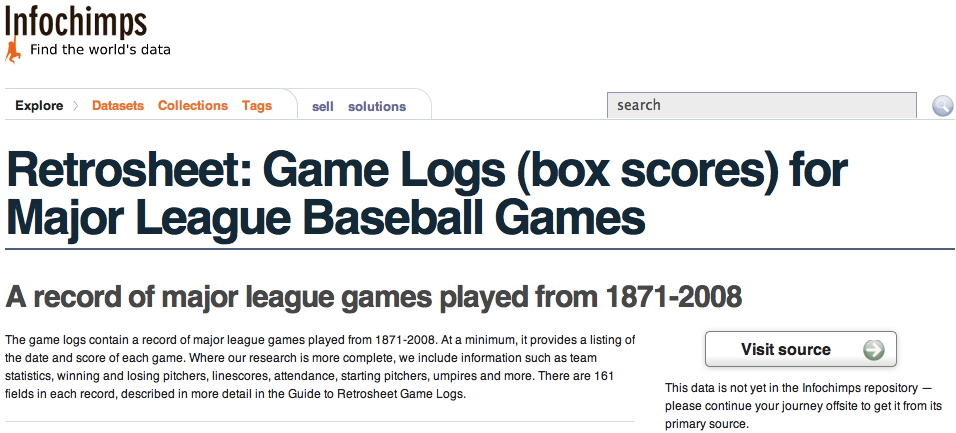
\includegraphics[width=6.5cm]{images/game_logs.png}
    \end{columns}}
\end{frame}

\begin{frame}[fragile]
    \frametitle{Infochimps API}
    \fbox{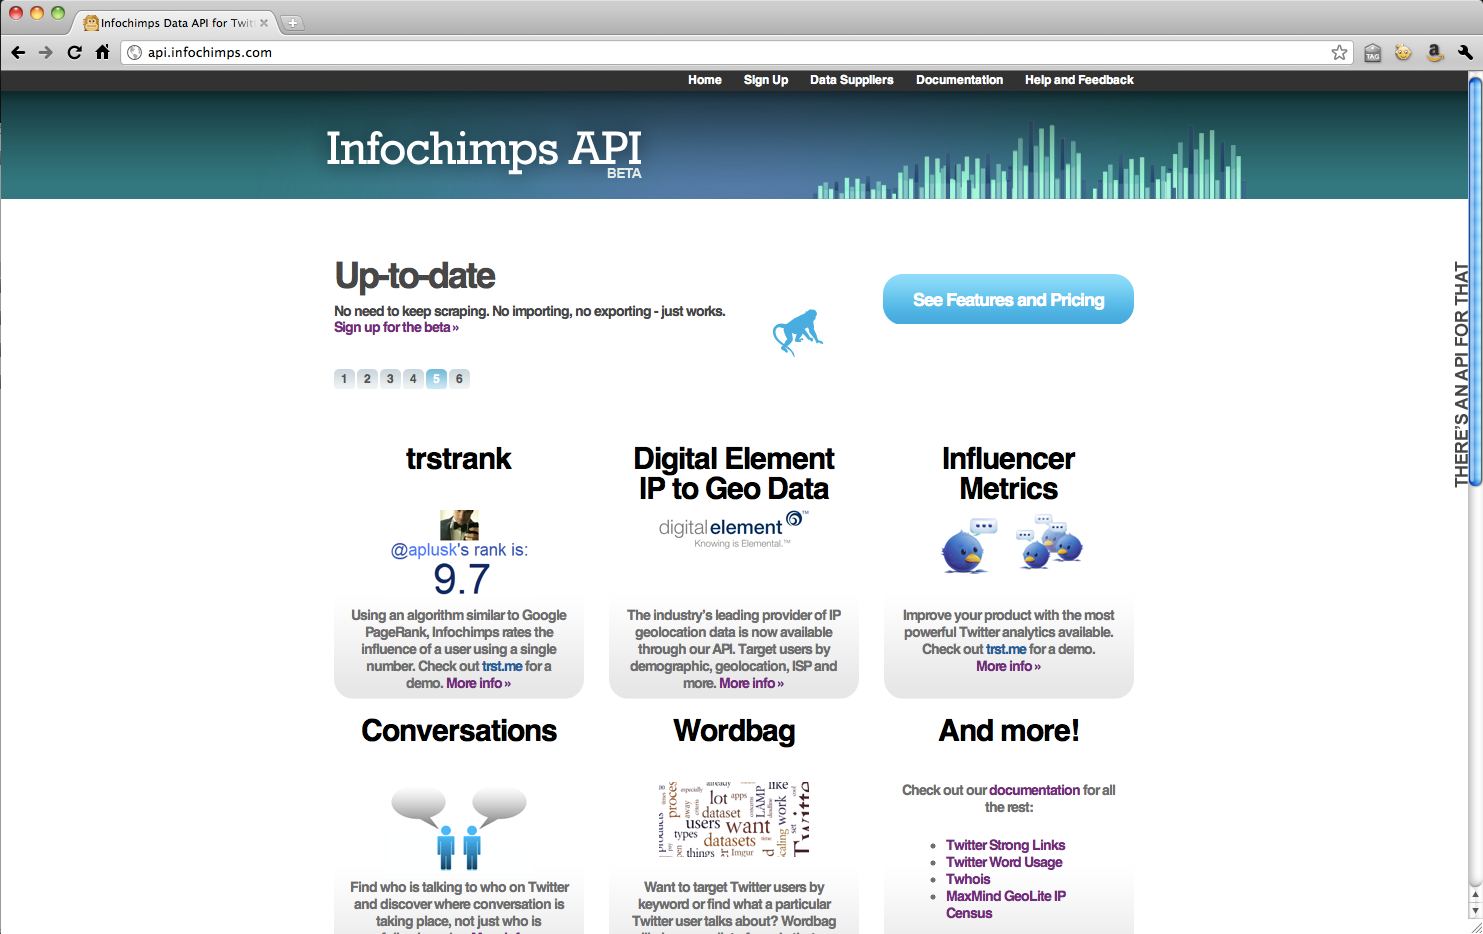
\includegraphics[width=11cm]{images/infochimps_screenshot.png}} \\
    \vspace{2mm}
    \uncover<2->{For more info see vid by Flip Kromer: \url{http://vimeo.com/16819171}}
\end{frame}

% section introduction_to_infochimps (end)

\section{The \texttt{infochimps} R package} % (fold)
\label{sec:infochimps_r_package}

\begin{frame}[fragile]
    \frametitle{\texttt{infochimps} R package}
    \textbf{Idea}: create functions for every API call to integrate querying in \texttt{R}
        \begin{itemize}
            \item My first package accepted to CRAN!
            \item \url{http://cran.r-project.org/web/packages/infochimps/}
            \item  Update as new ones API calls roll-out
        \end{itemize}
        \uncover<2->{Inspired by other R API wrappers
        \begin{itemize}
            \item \href{http://cran.r-project.org/web/packages/twitteR/}{\texttt{twitteR}} by Jeff Gentry
            \item \href{http://cran.r-project.org/web/packages/IBrokers/}{\texttt{iBrokers}} by Jeffrey Ryan
            \item \href{http://cran.r-project.org/src/contrib/Archive/nytR/}{\texttt{nytR}} by Shane Conway (archived)
        \end{itemize}}
        \uncover<3->{\begin{columns}
            \column{.5\textwidth}
                \begin{block}{Twitter related}
                    \begin{itemize}
                        \item \texttt{conversations}
                        \item \texttt{influence}
                        \item \texttt{strong.links}
                        \item \texttt{trstrank}
                        \item \texttt{word.bag}
                        \item \texttt{word.stats}
                    \end{itemize}
                \end{block}
            \column{.5\textwidth}
                \begin{block}{Geo-location related}
                    \begin{itemize}
                        \item \texttt{census}
                        \item \texttt{demographics}
                        \item \texttt{domain}
                        \item \texttt{ip.geo}
                    \end{itemize}
                \end{block}
                \vspace{8.5mm}
        \end{columns}}
\end{frame}

\begin{frame}[fragile]
    \frametitle{Basic usage framework}
    \begin{center}
        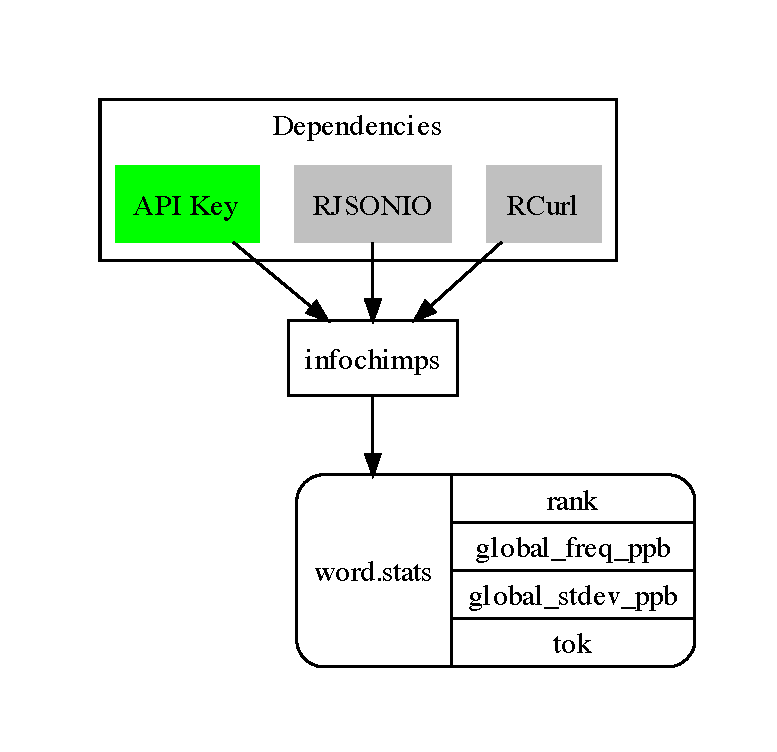
\includegraphics[width=8cm]{images/struct.pdf}
    \end{center}
\end{frame}

\begin{frame}[fragile]
    \frametitle{My first \texttt{infochimps} call}
    \alert<1>{Generate \texttt{infochimps} session}
    \begin{lstlisting}
> library(infochimps)
> my.api<-``some.long.alpha.numeric''
> ic<-infochimps(my.api)
    \end{lstlisting}
    \alert<2>{Get statistics for word ``data''}
    \begin{lstlisting}
> data.stats<-word.stats(``data'',ic)
> print(data.stats)
$global_stdev_ppb
[1] 2376464

$range
[1] 0.01266617

$tok
[1] ``data''

$global_freq_ppb
[1] 151562.4
    \end{lstlisting}
\end{frame}

\begin{frame}[fragile]
    \frametitle{The \texttt{word.stats} function}
    \begin{lstlisting}[language=R]
word.stats <-
function(tok,session) {
    word.url<-paste(session$base,"word_stats.json?tok=",
        tok,"&apikey=",session$api.key,sep="")
    word.get<-getURL(word.url)
    word.data<-fromJSON(word.get)
    # Simple error checking
    if(is.null(word.data$error)) {
        return(word.data)
    }
    else {
        warning(word.data$message[[1]])
        return(NA)
    }
}    
    \end{lstlisting}
    \uncover<2->{\alert<2>{All function follow this basic framework}}
\end{frame}


% section infochimps_r_package (end)

\section{Blog hits map} % (fold)
\label{sec:blog_hits_map}

\begin{frame}[fragile]
    \frametitle{Visualizing the location of blog visitors}
    The \texttt{ip.geo} function provides detailed geo-location data for a given IP address
    \begin{itemize}
        \item City, metro, country and continent codes (with confidence)
        \item Zip codes
        \item Latitude/Longitude
        \item Much more...
    \end{itemize}
    \uncover<2->{Using web log data from \url{http://drewconway.com/zia}, visualize one days worth of blog hits
    \begin{enumerate}
        \item Parse log file by IP address and date/time
        \item Use \texttt{ip.geo} to find lat/long for each hit
        \item Plot on map using \texttt{ggplot2}
    \end{enumerate}}
\end{frame}

\begin{frame}[fragile]
    \frametitle{Step 1: Parse log file}
    \scriptsize{\begin{lstlisting}[language=R]
# Load libraries
library(infochimps)
library(ggplot2)
library(maps)

# Need to load and clean the data
log.data<-read.delim("data/drewconway_com-Dec-2010.txt", 
    sep="-", header=FALSE, as.is=TRUE)
log.data<-data.frame(list("IP"=log.data$V1, "Date.Time"=log.data$V3, 
    "Log"=log.data$V4), stringsAsFactors=FALSE)
log.data$IP<-gsub(" ","", log.data$IP)

# First, get the dates in useable format
log.data$Date.Time<-gsub("[\\[ ]","",log.data$Date.Time)
log.data$Date.Time<-strptime(log.data$Date.Time, format="%d/%b/%Y:%H:%M:%S ")

# Filter out only those logs accessing the right blog post
log.data<-log.data[grep("(\\?p\\=|index\\.php)",log.data$Log),]
    \end{lstlisting}}
\end{frame}

\begin{frame}[fragile]
    \frametitle{Step 2: Get lat/long data}
    \scriptsize{\begin{lstlisting}[language=R]
# Create infochimps session
api.key<-"my.long.alpha.numeric"
ic<-infochimps(api.key)

# Get lattitude and longitude data for all of the IPs
ips<-unique(log.data$IP)

get.latlong<-function(ip) {
    geo.data<-ip.geo(ip,ic)
    return(c(ip, geo.data$lat,geo.data$longitude))
}

# Create data frame to merge into log data
geo.data<-lapply(ips, get.latlong)  
geo.df<-as.data.frame(do.call("rbind", geo.data),stringsAsFactors=FALSE)
names(geo.df)<-c("IP","Latitude","Longitude")
log.geo<-merge(log.data,geo.df,by="IP")
log.geo$Latitude<-as.numeric(log.geo$Latitude)
log.geo$Longitude<-as.numeric(log.geo$Longitude)

# Create counts, and sort chronologically
log.count<-ddply(log.geo,.(IP, Date.Time, Latitude, Longitude), 
    summarise, Count=length(Log))
log.count<-log.count[with(log.count, order(Date.Time)),]
    \end{lstlisting}}
\end{frame}

\begin{frame}[fragile]
    \frametitle{Step 3: Visualize on global map}
    \scriptsize{\begin{lstlisting}[language=R]
# Ready to visualize
world.map<-data.frame(map(plot=FALSE)[c("x","y")])

# Create frame for every second in data
plot.num<-1
for(d in strftime(log.count$Date.Time)) {
    log.sub<-log.count[which(strftime(log.count$Date.Time)==d),]
    geo.plot<-ggplot(world.map, aes(x=x,y=y))+geom_path(aes(colour=``grey''))
    geo.plot<-geo.plot+geom_point(data=log.sub, aes(x=Longitude, y=Latitude, 
            color=``red'', alpha=0.75, size=Count))+
        annotate(``text'',x=-125,y=-5,label=strftime(d, format=``%H:%M:%S''))+
        theme_bw()+scale_colour_manual(values=c(``grey''=``grey'',``red''=``red''),
            legend=FALSE)+
        scale_alpha(legend=FALSE)+scale_size(legend=FALSE)+
            coord_map(projection=``lagrange'',ylim=c(-40,70),xlim=c(-145,155))+
        opts(panel.grid.major=theme_blank(),axis.ticks=theme_blank(),
            axis.text.x=theme_blank(),axis.text.y=theme_blank())+
        xlab(``'')+ylab(``'')
    ggsave(plot=geo.plot,filename=paste(``images/maps/'',plot.num,``.png'',sep=``''),
        width=6,height=4)
    plot.num<-plot.num+1
}

# Run this at the command-line to join the files as a movie
# ffmpeg -f image2 -r 5 -i images/maps/%d.png -b 600k blogpost.mp4
    \end{lstlisting}}
\end{frame}

\begin{frame}[fragile]
    \frametitle{The movie}
    \begin{center}
        \includemovie[
            poster,
            text={Blog hits map}
        ]{9cm}{7cm}{../blogpost.mp4}
    \end{center}
\end{frame}

% section blog_hits_map (end)

\section{Programming languages on Twitter} % (fold)
\label{sec:comparison_of_programming_language_tweeting}

\begin{frame}[fragile]
    \frametitle{How do people tweet about different languages?}
    \begin{center}
        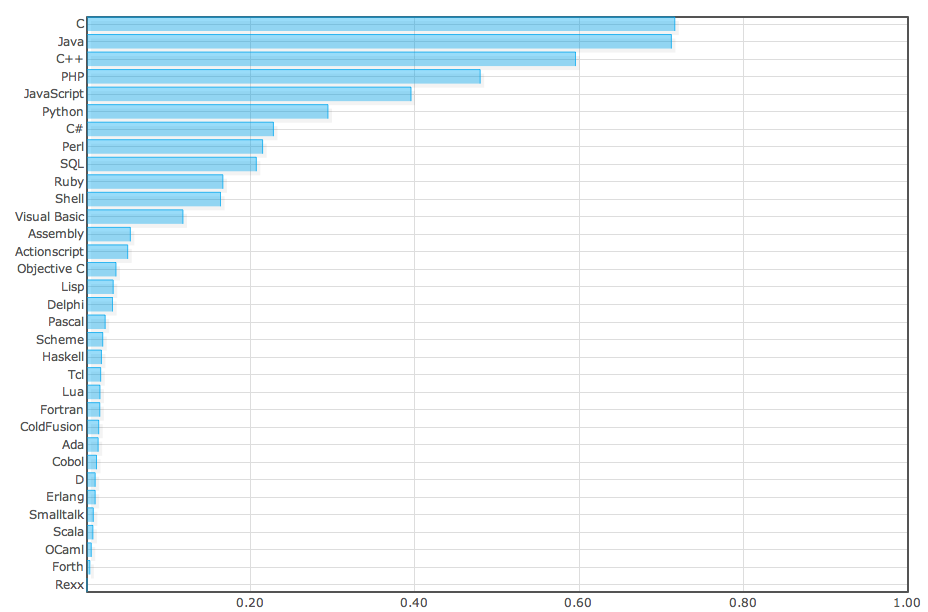
\includegraphics[width=10cm]{images/lang_pop.png}
    \end{center}
    \begin{tabular}{r}
        \hline \\
        \scriptsize{Source: \url{http://langpop.com/},  Last updated Sat Nov 27 08:45:50}
    \end{tabular}
\end{frame}

\begin{frame}[fragile]
    \frametitle{Use the \texttt{word.stats} function}
    The \texttt{word.stats} function returns token frequency data
    \begin{itemize}
        \item Global frequency (parts per-billion)
        \item Standard deviation of frequency (parts per-billion)
        \item Range (normalized number of unique users who have used it)
    \end{itemize}
    \uncover<2->{Use the global frequency to create chart for Twitter mentions
    \begin{enumerate}
        \item Create vector of computer languages
        \item User \texttt{word.stats} to collect frequency data
        \item Plot bar chat with \texttt{ggplot2}
    \end{enumerate}}
    \uncover<3->{\alert{Disadvantage}: cannot get stats for languages like C, C#, C++}
\end{frame}

\begin{frame}[fragile]
    \frametitle{Getting the data}
    \scriptsize{\begin{lstlisting}[language=R]
# rogramming languages
prog.langs<-c("java","php","javascript","python","sql","perl","ruby",
    "actionscript","assembly","lisp","delphi","pascal","scheme","haskell",
    "tcl","lua","fortran","coldfusion","ada","cobol","erlang","smalltalk",
    "scala","ocaml","forth","rexx","rstats")
    
# Get word stats for all languages
lang.stats<-lapply(prog.langs,function(t) unlist(word.stats(t,ic)))
lang.df<-as.data.frame(do.call("rbind",lang.stats), stringsAsFactors=FALSE)
lang.df$global_stdev_ppb<-as.numeric(lang.df$global_stdev_ppb)
lang.df$range<-as.numeric(lang.df$range)
lang.df$global_freq_ppb<-as.numeric(lang.df$global_freq_ppb)

# Dummy for common words
common<-rep(0,nrow(lang.df))
common[match(c("ruby","assembly","lisp","scheme","ada","forth"),lang.df$tok)]<-1
lang.df$common<-as.factor(common)

# Sort by frequency
lang.df<-lang.df[with(lang.df, order(global_freq_ppb)),]
    \end{lstlisting}}
\end{frame}

\begin{frame}[fragile]
    \frametitle{Visualizing computer languages mentioned on Twitter}
    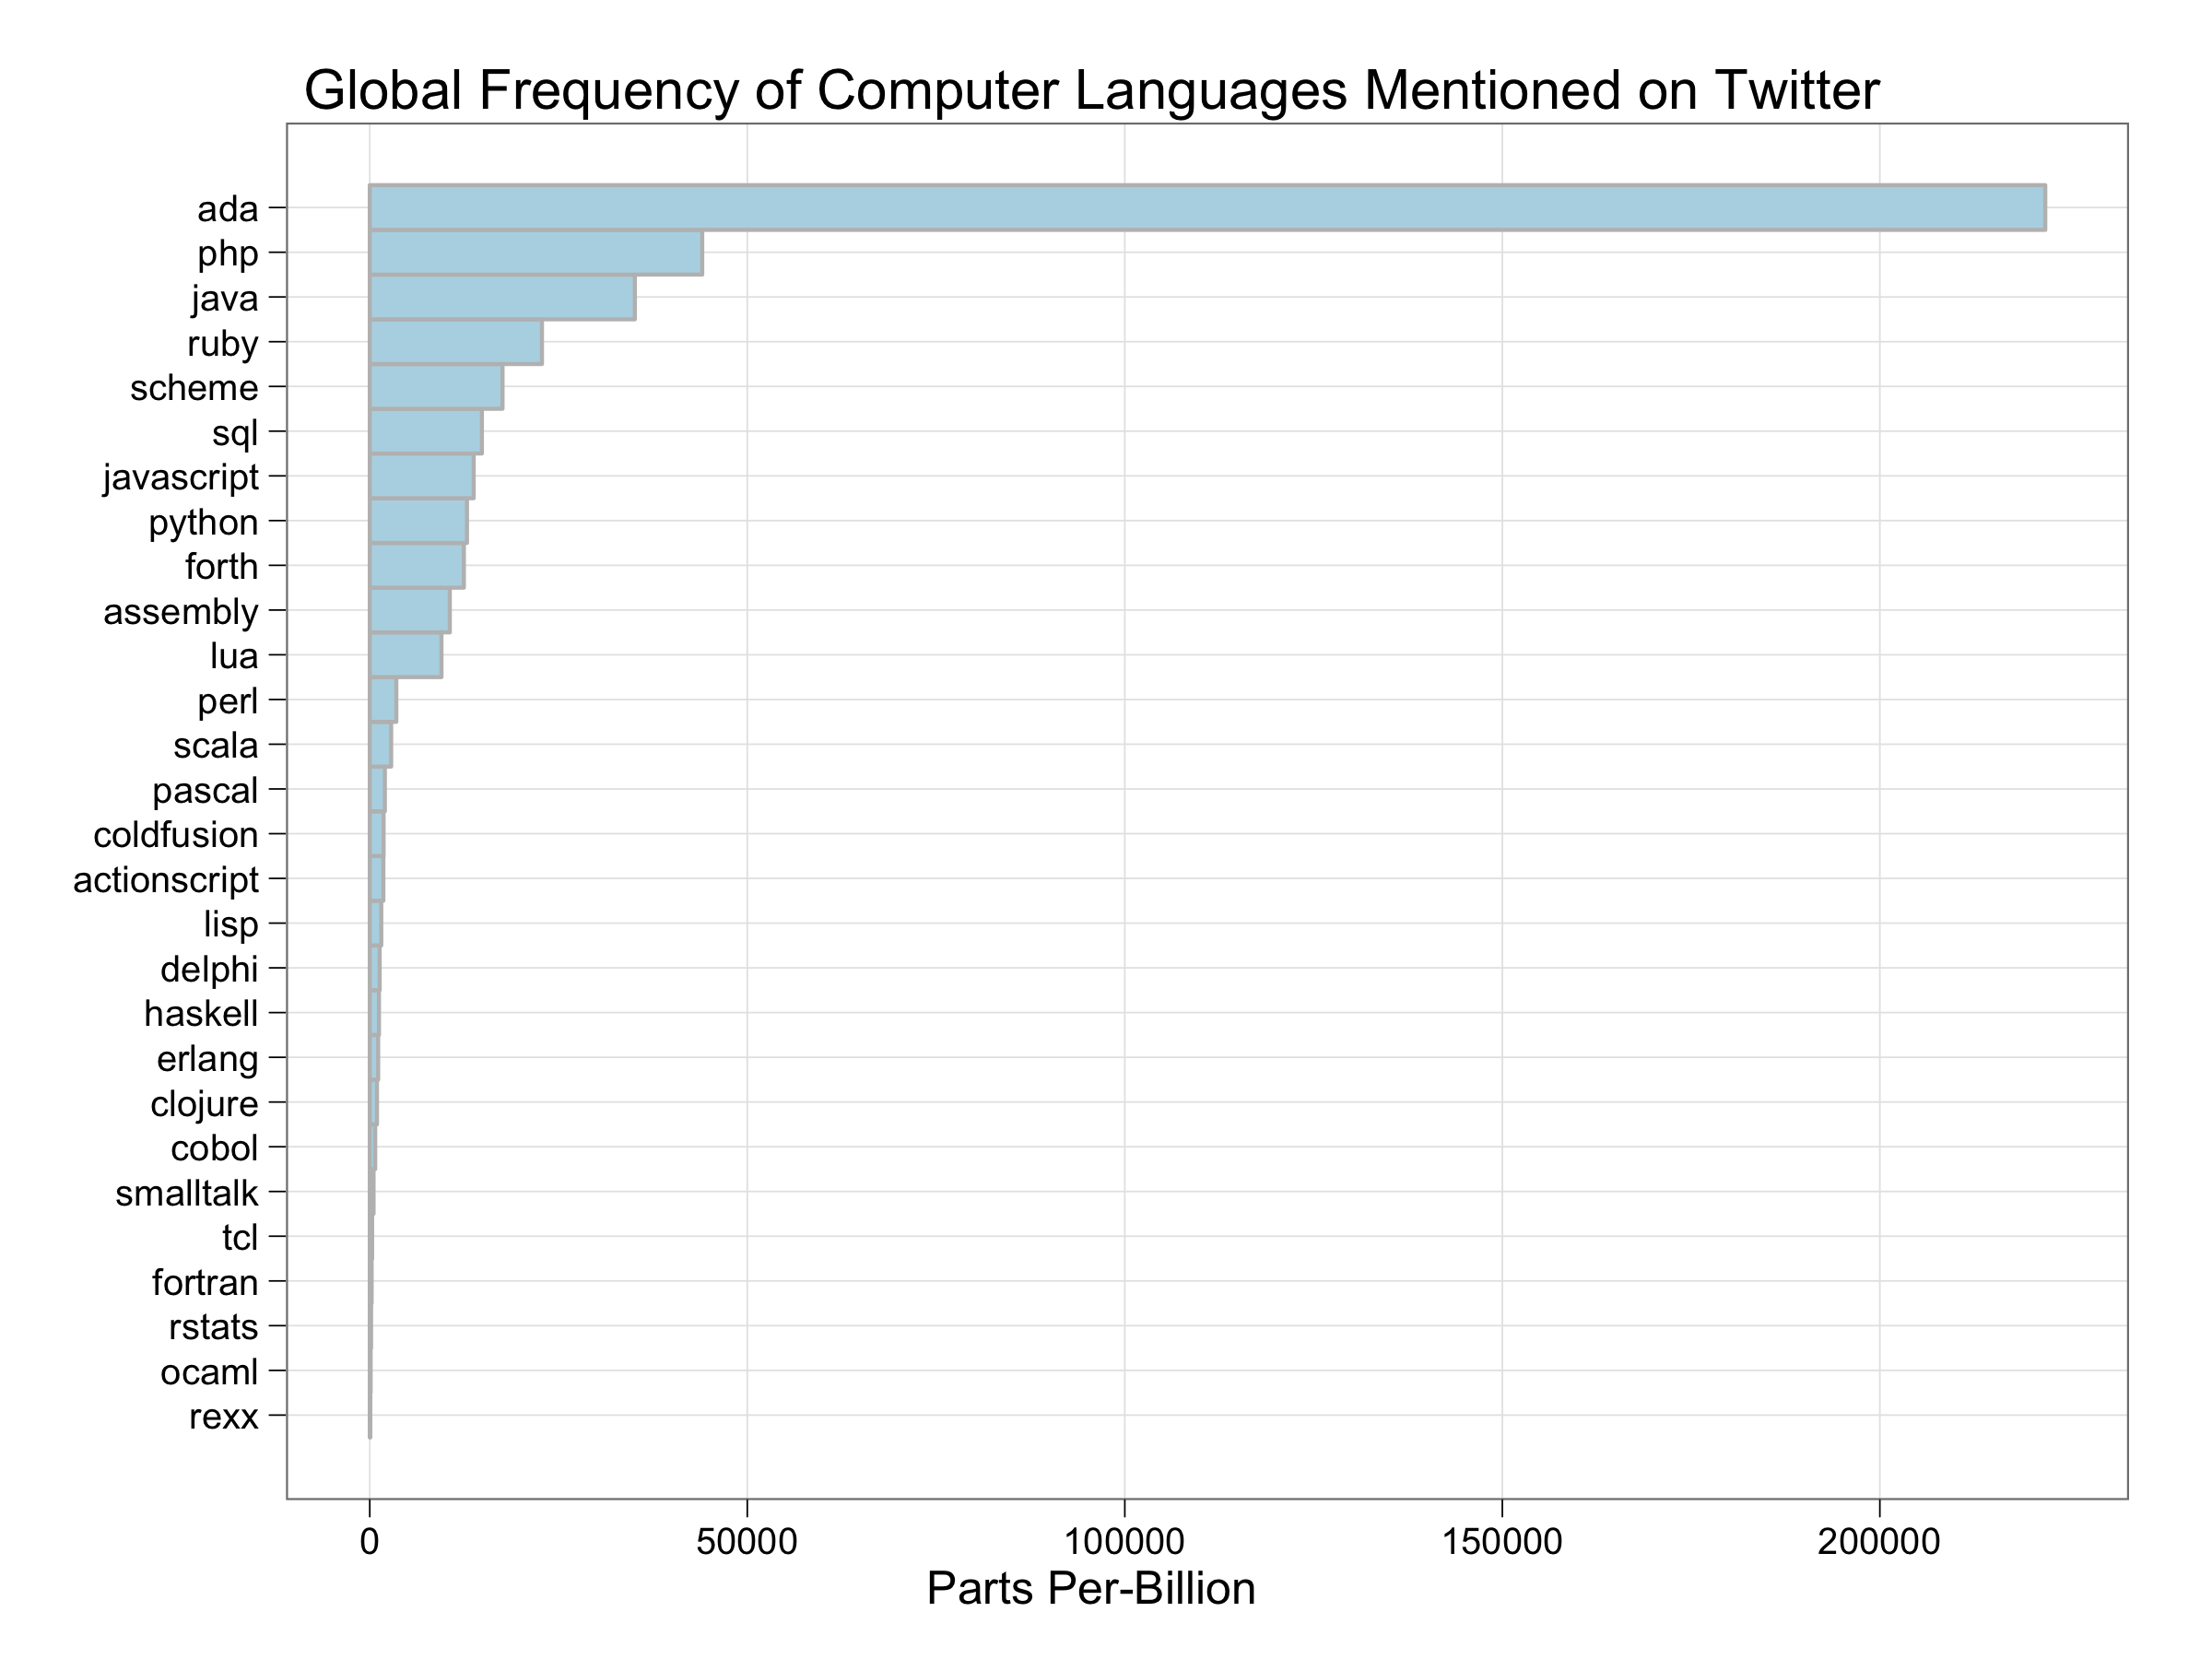
\includegraphics[width=10cm]{images/lang_pop1.png}
\end{frame}

\begin{frame}[fragile]
    \frametitle{Ambiguous terms}
    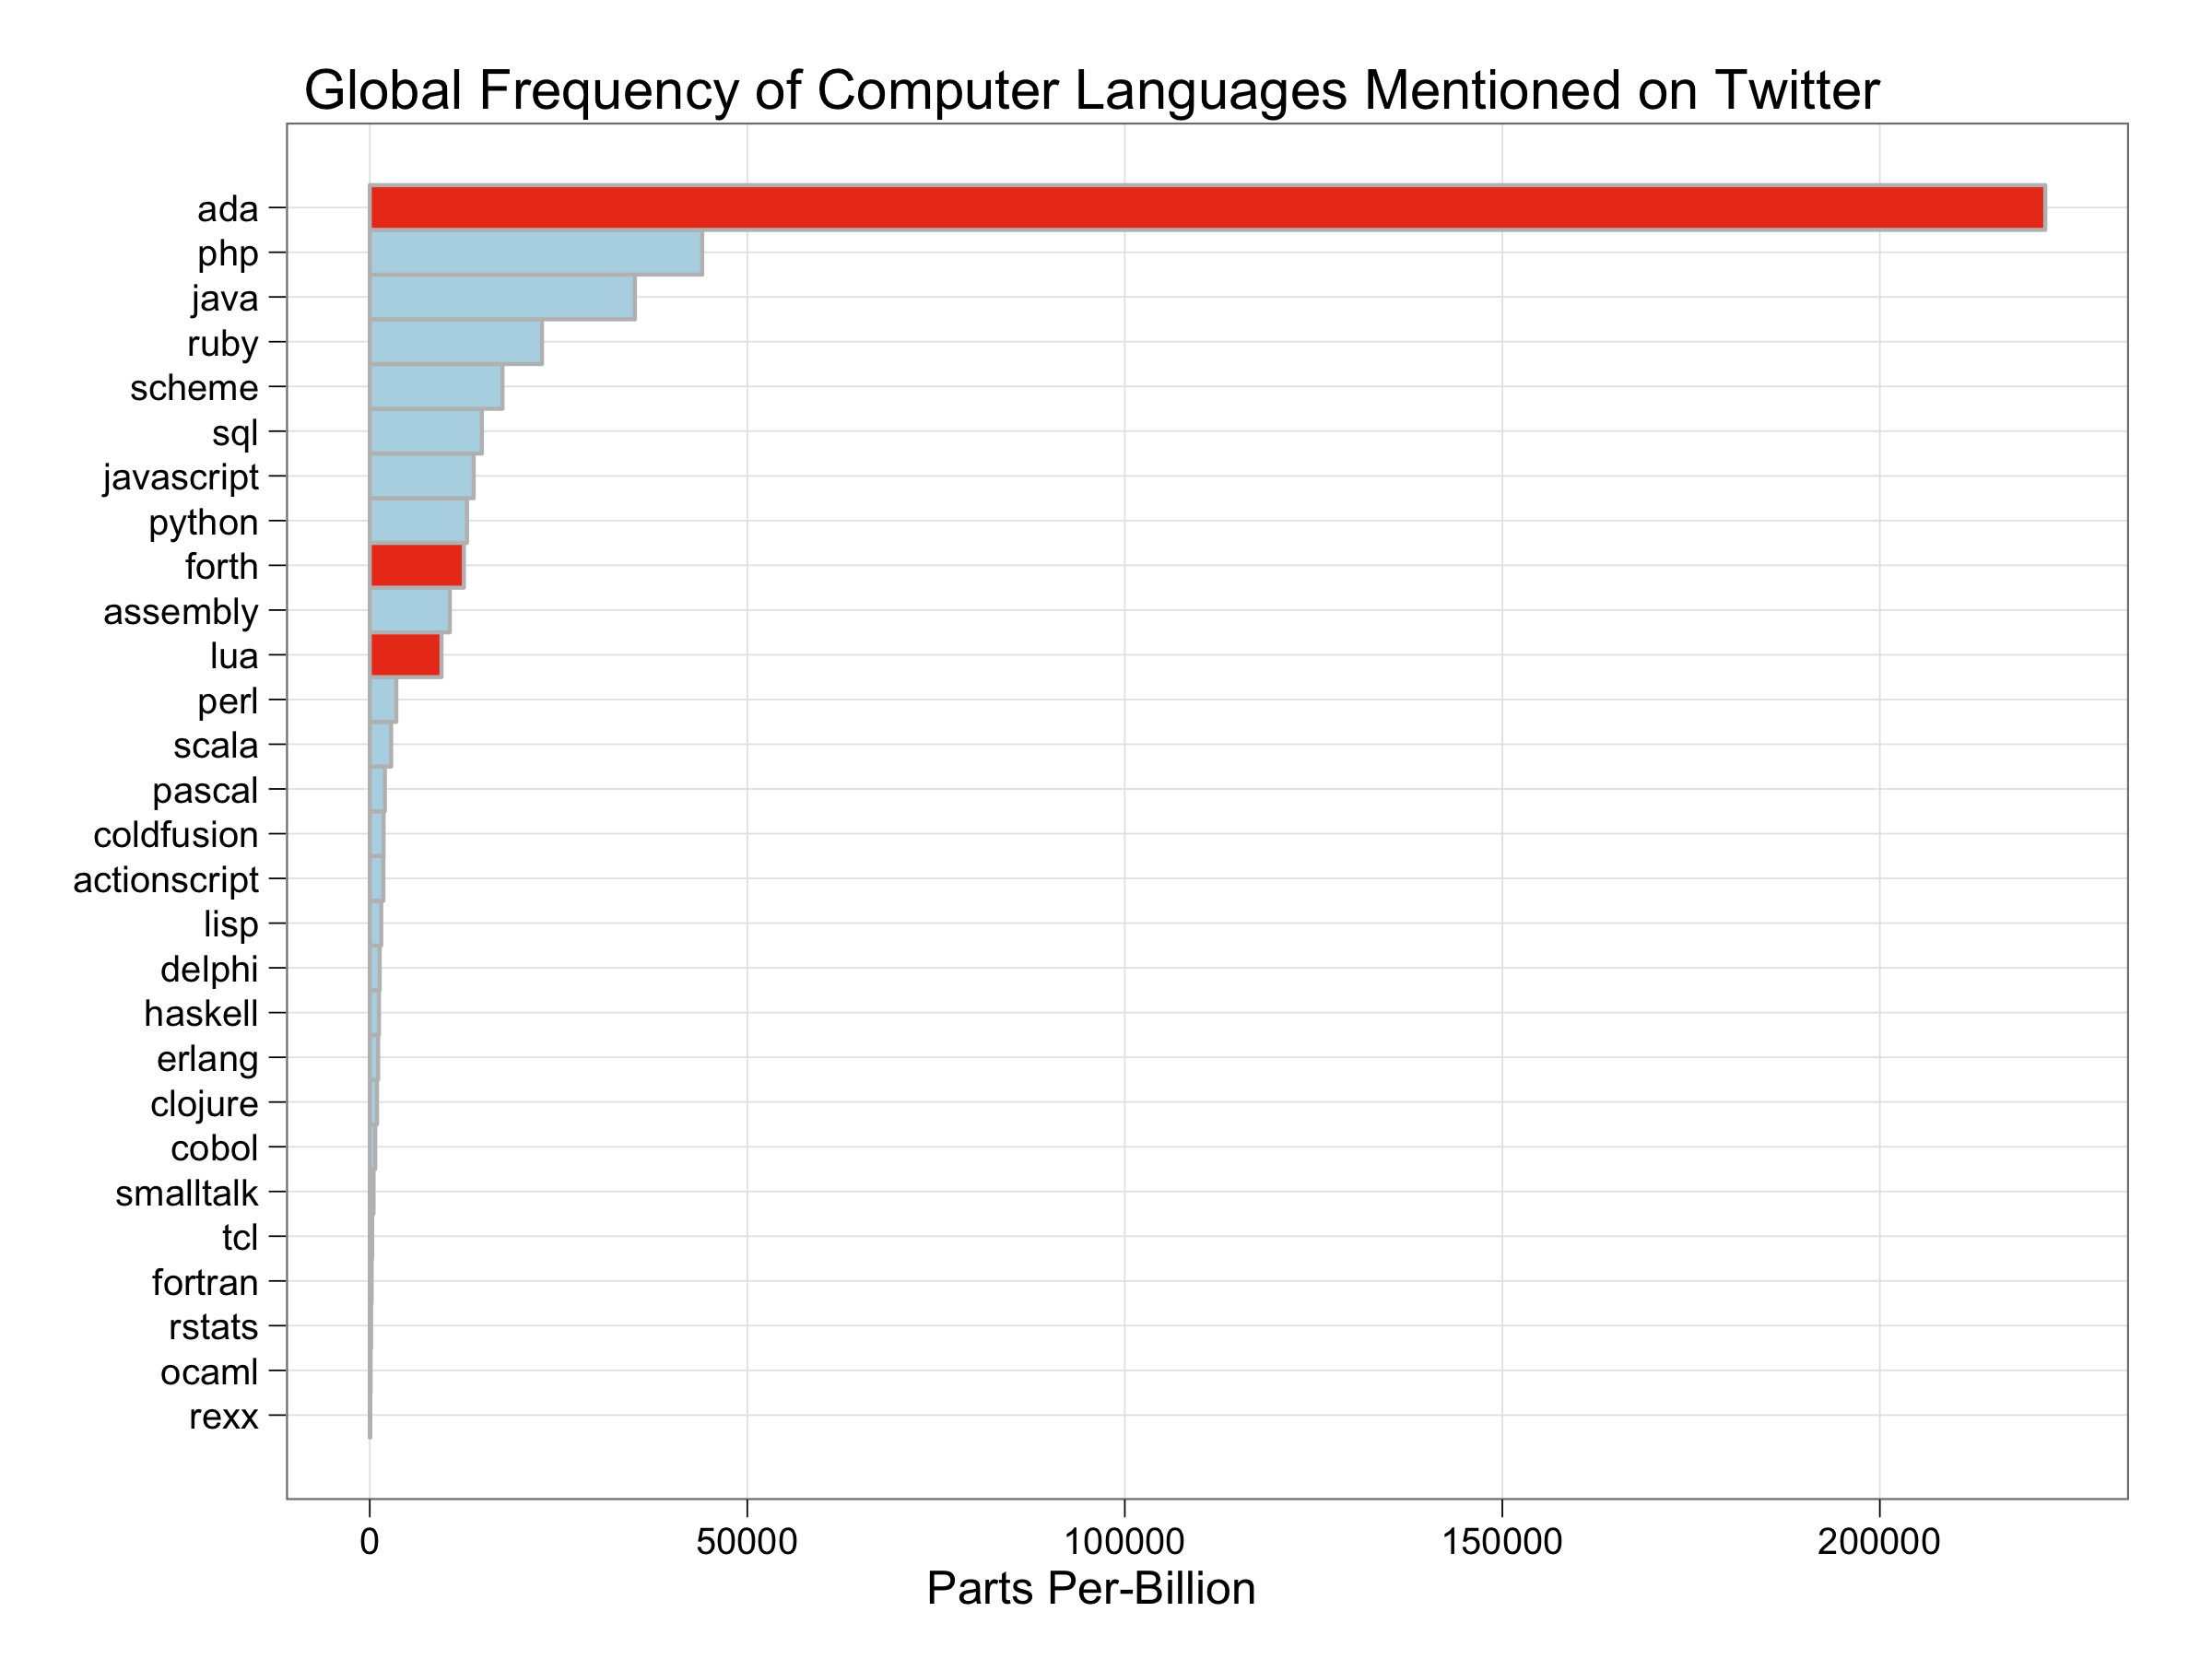
\includegraphics[width=10cm]{images/lang_pop2.png}
\end{frame}

\begin{frame}[fragile]
    \frametitle{Terms cleans and logs taken}
    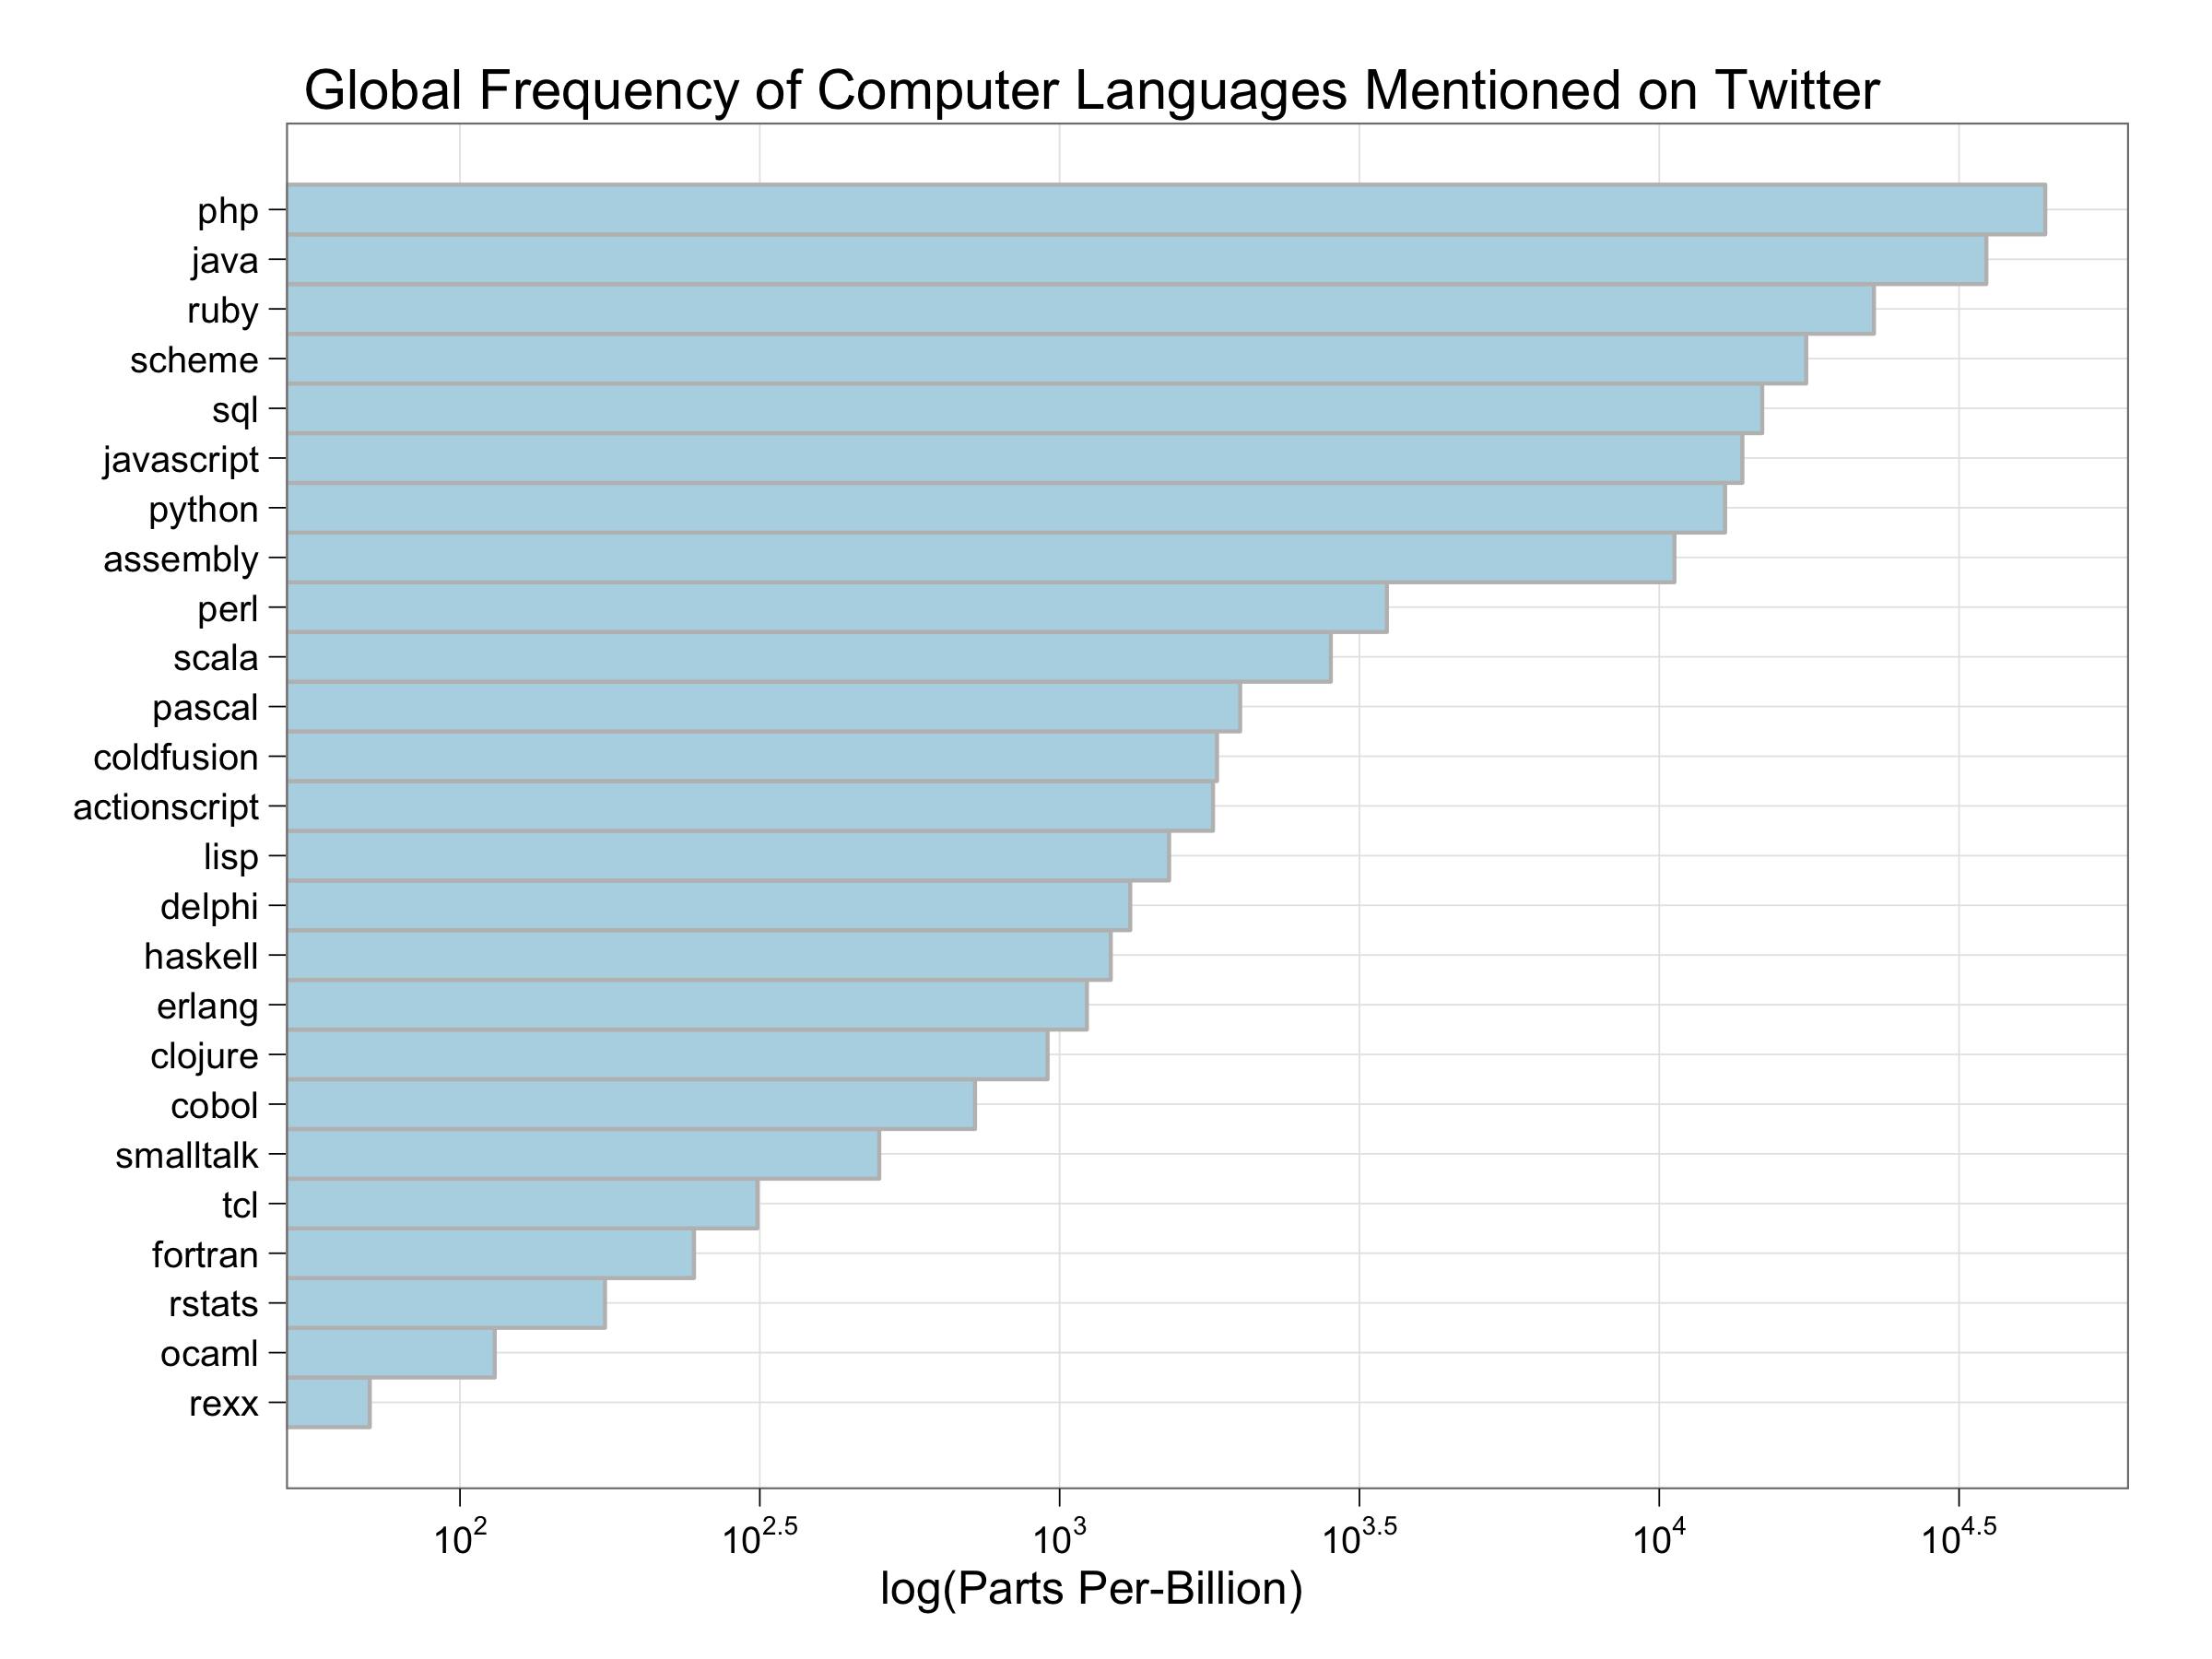
\includegraphics[width=10cm]{images/lang_pop3.png}
\end{frame}

% section comparison_of_programming_language_tweeting (end)

\begin{frame}[fragile]
    \frametitle{Thank You!}
    \begin{tabular}{ll}
        E-mail: & drew.conway@nyu.edu \\
        Web:    & \url{http://drewconway.com/zia} \\
        Twitter:& @drewconway
    \end{tabular}
    \vspace{2cm} \\
    Example code and slides available at \url{https://github.com/drewconway/infochimps/tree/master/examples}
\end{frame}

\end{document}
